\documentclass[../../../../main.tex]{subfiles}
\usepackage{tikz}
\usetikzlibrary{patterns}

\begin{document}
\section*{京都大学 1995年 前期}

\subsection*{第1問}

\subsection*{第2問}
[解] $a, b \in \mathbb{N}, a > b \cdots \text{\textcircled{1}}$\\
$p, d \in \text{prime} \quad p > 2 \cdots \text{\textcircled{2}}$

$A = a^p - b^p$ とおく。\\
$A = (a - b)(a^{p-1} + \cdots + b^{p-1})$\\
であり、$a - b \in \mathbb{N}$、$a^{p-1} + \cdots + b^{p-1} \ge 2$（$\because \text{\textcircled{1}}$）から、$A \in \text{prime}$ には $a - b = 1 \iff a = b + 1$ が必要。以下、$A-1 = (b+1)^p - b^p - 1$ が $2p$ でわり切れることを示す。$\cdots \bigstar$

$1^\circ \ A - 1 \equiv 0 \pmod 2$ の証明\\
$(b+1)^p, (b^p)$ の偶奇は一致するから、$A - 1 \equiv 0 \pmod 2$ （終）

$2^\circ \ A - 1 \equiv 0 \pmod p$ の証明\\
$r = 1, 2, 3, \cdots, p-1$ の時、
\[
{}_p\mathrm{C}_r = \frac{p}{r} {}_{p-1}\mathrm{C}_{r-1} \in \mathbb{Z}
\]
において、$r$ は $p$ と互いに素だから、${}_p\mathrm{C}_r$ は $p$ の倍数である。\\
から
\[
A - 1 = {}_p\mathrm{C}_1 b^{p-1} + \cdots + {}_p\mathrm{C}_{p-1} b \equiv 0 \pmod p \quad \text{（終）}
\]
$1^\circ, 2^\circ, p>2$ から $A-1$ は $2p$ でわりきれる（終）

[別解]\\
（フェルマーの小定理を証明した上で）以下
\[
a^p - b^p \equiv a - b \equiv 1 \pmod p
\]

\framebox{
\begin{minipage}{0.9\textwidth}
[フェルマーの小定理の証明の再掲]\\
\textcircled{1} ウィルソンを経由
\begin{align*}
a \cdot 2a \cdot 3a \cdots (p-1)a &\equiv 1 \cdot 2 \cdots (p-1) \pmod p \\
(p-1)! \cdot a^{p-1} &\equiv (p-1)! \pmod p \\
a^{p-1} &\equiv 1 \pmod p
\end{align*}

\textcircled{2} 帰納法（$n^p \equiv n$）\\
(ア) $(m+1)^p \equiv m^p + 1 \pmod p$ を用いる方法と\\
(イ) $(x+y)^p \equiv x^p + y^p \pmod p$ から
\[
a^p = (1 + \cdots + 1)^p \equiv \cdots \equiv 1 + 1 + \cdots + 1 = a
\]
とする方法
\end{minipage}
}

\subsection*{第3問}
[解] 3交点の $x$ 座標を、小さい順に $\alpha, \beta, \gamma$ とおく。\\
又、$f(x) = ax^2 + bx + c$ とする。
\[
x^3 - f(x) = (x-\alpha)(x-\beta)(x-\gamma) \cdots \text{\textcircled{1}}
\]
各点での接線を $l_1, l_2, l_3$ として、これらは
\[
y = 3k^2 x - 2k^3 \quad (k=\alpha, \beta, \gamma) \cdots \text{\textcircled{2}}
\]
で表される。\textcircled{2} が $P$ を通ることから
\[
2k^3 - 3pk^2 + q = 0 \cdots \text{\textcircled{3}}
\]
したがって、$\alpha, \beta, \gamma$ は $k$ の3次式 \textcircled{3} の3実解で、\textcircled{1} から
\[
x^3 - f(x) = x^3 - \frac{3}{2}p x^2 + \frac{q}{2}
\]
係数比較して
\[
a = \frac{3}{2}p, \quad b = 0, \quad c = -\frac{q}{2} \cdots (1)
\]

(2) $p, q$ の条件は $x$ の3次方程式 $x^3 - \frac{3}{2}px^2 + \frac{q}{2} = 0 \cdots \text{\textcircled{4}}$ が3異実解を持つこと。\textcircled{4} の左辺 $g(x)$ とおく。$g'(x) = 3x^2 - 3px$ から、$p$ によって下のように分かれる

$1^\circ \ p = 0$ の時\\
$g'(x) \ge 0$ となり、$g(x)$ は単調増加し、\textcircled{4} が3異実解を持つことはない。

$2^\circ \ p > 0$ の時\\
\begin{center}
\begin{tabular}{|c|c|c|c|c|c|}
\hline
$x$ & $\cdots$ & $0$ & $\cdots$ & $p$ & $\cdots$ \\
\hline
$g'$ & $+$ & $0$ & $-$ & $0$ & $+$ \\
\hline
$g$ & $\nearrow$ & & $\searrow$ & & $\nearrow$ \\
\hline
\end{tabular}
\end{center}
上図から、条件は
\begin{align*}
& g(0) > 0 \land g(p) < 0 \\
\iff & \frac{q}{2} > 0 \land - \frac{p^3}{2} + \frac{q}{2} < 0 \\
\iff & q > 0 \land -p^3 + q < 0
\end{align*}

$3^\circ \ p < 0$ の時\\
$2^\circ$ と同様に、条件は
\[
g(p) > 0 \land g(0) < 0 \iff q < 0 \land -p^3 + q > 0
\]

以上まとめて
\[
\begin{cases}
p > 0, \quad 0 < q < p^3 \\
\text{又は} \\
p < 0, \quad p^3 < q < 0
\end{cases}
\]

\subsection*{第4問}

\subsection*{第5問}
[解] (1) 題意のようになるのは、1人目がどちらの席にすわるか場合分けして考えて、確率 $P_1$ として
\[
P_1 = \frac{1}{12} \cdot \frac{2}{10} + \frac{2}{12} \cdot \frac{1}{8} = \frac{9}{240} = \frac{3}{80} \quad \text{（終）}
\]

(2) 席のうまる順番は
\begin{align*}
& 1^\circ \ (2, 4, 6) \quad (6, 4, 2) \cdots \text{\textcircled{1}} \\
& 2^\circ \ (2, 6, 4) \quad (6, 2, 4) \cdots \text{\textcircled{2}} \\
& 3^\circ \ (4, 2, 6) \quad (4, 6, 2) \cdots \text{\textcircled{3}}
\end{align*}
2と6の対称性から、\textcircled{1}, \textcircled{2}, \textcircled{3} の2つの順番がおこる確率は、いずれも等しく、排反だから、これらのおこる確率の和がもとめる確率 $P_2$ である\\
\textcircled{1} の時 $\frac{2}{12} \cdot \frac{2}{9} \cdot \frac{2}{6} = \frac{1}{81}$ \\
\textcircled{2} の時 $\frac{2}{12} \cdot \frac{2}{9} \cdot \frac{2}{6} = \frac{1}{81}$ \\
\textcircled{3} の時 $\frac{2}{12} \cdot \frac{2}{8} \cdot \frac{2}{6} = \frac{1}{72}$ \\
より、
\[
P_2 = 2 \left( \frac{1}{81} + \frac{1}{81} + \frac{1}{72} \right) = \frac{25}{324} \quad \text{（終）}
\]

\subsection*{第6問}
[解] 時刻 $t$ での水深 $h$、水表面積 $S$ とおくと
\begin{align*}
V &= S \frac{dh}{dt} \cdots \text{\textcircled{1}} \\
S &= V t + \pi a^2 \\
&= \pi f(h)^2 \cdots \text{\textcircled{2}}
\end{align*}

\begin{center}
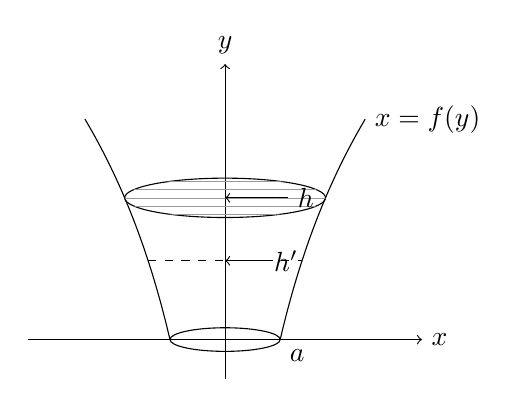
\begin{tikzpicture}
  \draw[->] (-2.5, 0) -- (2.5, 0) node[right] {$x$};
  \draw[->] (0, -0.5) -- (0, 3.5) node[above] {$y$};
  
  \draw[domain=0:2.8, variable=\y, smooth] plot ({0.7*exp(\y/3)}, \y) node[right] {$x=f(y)$};
  \draw[domain=0:2.8, variable=\y, smooth] plot ({-0.7*exp(\y/3)}, \y);
  
  \draw (0,0) ellipse (0.7 and 0.15);
  \node[below right] at (0.7,0) {$a$};
  
  \draw (0, 1.8) ellipse ({0.7*exp(1.8/3)} and 0.25);
  \fill[pattern=horizontal lines, pattern color=gray!80] (0, 1.8) ellipse ({0.7*exp(1.8/3)} and 0.25);
  
  \draw[<-] (0, 1.8) -- (0.8, 1.8) node[right] {$h$};
  \draw[<-] (0, 1.0) -- (0.5, 1.0) node[right] {$h'$};
  \draw[dashed] ({-0.7*exp(1.0/3)}, 1.0) -- ({0.7*exp(1.0/3)}, 1.0);
\end{tikzpicture}
\end{center}

\textcircled{2} と $f(y) > 0$ から
\[
f(h) = \sqrt{a^2 + \frac{V}{\pi}t} \cdots \text{\textcircled{3}}
\]

\textcircled{2} を \textcircled{1} に代入、セパレして
\[
\frac{V}{Vt + \pi a^2} dt = dh
\]
積分して、$C$ を定数とすると
\[
\log \left( t + \frac{\pi}{V} a^2 \right) = h + C
\]
$t=0$ で $h=0$ だから、$C = \log \frac{\pi}{V} a^2$ なので、代入して
\begin{align*}
t &= e^h \cdot e^C - \frac{\pi}{V} a^2 \\
&= \frac{\pi}{V} a^2 (e^h - 1) \cdots \text{\textcircled{4}}
\end{align*}

$t=T$ で $h=h$ だから
\[
T = \frac{\pi}{V} a^2 (e^h - 1) \quad \text{（終）}
\]

\textcircled{4} を \textcircled{3} に代入し、$h$ を $y$ でおきかえて
\[
f(y) = a e^{\frac{y}{2}} \quad \text{（終）}
\]

\framebox{
\begin{minipage}{0.9\textwidth}
この時
\[
h' = \log \left( \frac{V t}{\pi a^2} + 1 \right), \quad S = \pi a^2 e^{h'} = \pi a^2 \left( \frac{V t}{\pi a^2} + 1 \right)
\]
より \textcircled{1} に代入
\[
V = (V t + \pi a^2) \cdot \frac{\pi a^2}{Vt + \pi a^2} \cdot \frac{V}{\pi a^2} = V
\]
$\implies$ あてそう
\end{minipage}
}
\end{document}
